\section{Beispiele für numerische Lösung nichtlinearer Gleichungssysteme}

\begin{example2}{Einleitendes Beispiel}

    \begin{minipage}{0.4\linewidth}
        Gesucht sind die Lösungen des Gleichungssystems:
    \end{minipage}
    \begin{minipage}{0.55\linewidth}
        \vspace{-6mm}
    $$f_1(x_1, x_2) = x_1^2 + x_2 - 11 = 0$$
    $$f_2(x_1, x_2) = x_1 + x_2^2 - 7 = 0$$
    \end{minipage}
    \vspace{1mm}\\
    Diese lassen sich interpretieren als die Nullstellen der Funktion:
    $$\textbf{f}: \R^2 \to \R^2 \quad \textbf{f}(x) = \begin{pmatrix} f_1 (x_1, x_2) \\ f_2 (x_1, x_2) \end{pmatrix} = \begin{pmatrix} x_1^2 + x_2 - 11 \\ x_1 + x_2^2 - 7 \end{pmatrix} = \begin{pmatrix} 0\\ 0 \end{pmatrix}$$
    Ein solches System lässt sich nicht in die Form $Ax = b$ bringen. 

    \begin{minipage}{0.5\linewidth}
    Geometrisch lassen sich die Lösungen als Schnittpunkte der beiden Funktionen interpretieren.\\
    Explizite Darstellung der Kurven:
    $$x_2 = 11 - x_1^2$$
    $$x_2 = \sqrt{7 - x_1}$$
    Schnittpunkte:
    $$\overline{\textbf{x}_1} = \begin{psmallmatrix} 3 \\ 2 \end{psmallmatrix}, \quad \overline{\textbf{x}_2} = \begin{psmallmatrix} -2.8 \\ 3.2 \end{psmallmatrix}$$
    $$\overline{\textbf{x}_3} = \begin{psmallmatrix} -3.8 \\ -3.3 \end{psmallmatrix}, \quad \overline{\textbf{x}_4} = \begin{psmallmatrix} 3.4 \\ -1.7 \end{psmallmatrix}$$
    \end{minipage}
    \begin{minipage}{0.5\linewidth}
    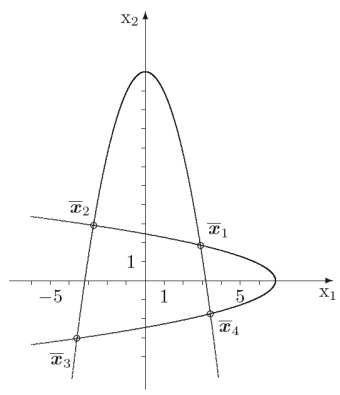
\includegraphics[width=\linewidth]{einleitendes_bsp_kap5.png}
    \end{minipage}
\end{example2}

\begin{example2}{Typbestimmung für Funktionen mehrerer Variablen}
    \begin{itemize}
        \item Addition: $f(x,y) = x + y$ \\ $\rightarrow$ skalarwertig, $\mathbb{R}^2 \rightarrow \mathbb{R}$
        \item Ohmsches Gesetz: $U(R,I) = R \cdot I$ \\ $\rightarrow$ skalarwertig
        \item Wurfweite: $W(v_0, \alpha) = \frac{v_0^2 \sin(2\alpha)}{g}$ \\ $\rightarrow$ skalarwertig
        \item Vektorwertige Funktion: $f(x_1, x_2, x_3) = \begin{psmallmatrix} x_1^2 + x_2^2 \\ x_1^2 + x_3^2 \\ x_2^2 + x_3^2 \\ x_1^2 + x_2^2 + x_3^2 \end{psmallmatrix}$
    \end{itemize}
    \end{example2}

    \begin{example2}{Zusammenhang mit der Elektrotechnik}
    \paragraph{Ohmsches Gesetz}
    Die an einem ohmschen Widerstand $R$ abfallende Spannung $U$ hängt vom Widerstand $R$ und der Stromstärke $I$ gemäss dem ohmschen Gesetz $U=R \cdot I$ ab. Also haben wir für die abhängige Variable $U=f(R, I)=R I$ die skalarwertige Funktion $f: \mathbb{R}^2 \longrightarrow \mathbb{R}$ mit den unabhängigen Variablen $R$ und $I$. Häufig schreibt man auch direkt
    $$
    U=U(R, I)=R \cdot I
    $$
    und bringt dadurch die Abhängigkeit der Variable $U$ von den unabhängigen Variablen $R$ und $I$ zum Ausdruck, wie wir es auch bereits vom eindimensionalen Fall kennen, z.B. $y=y(x)$.

    \paragraph{Reihenschaltung von Widerständen}
    Bei der Reihenschaltung von $n$ ohmschen Widerständen $R_1, R_2, \ldots, R_n$ ergibt sich der Gesamtwiderstand $R$ gemäss
    $$
    R=R(R_1, R_2, \ldots, R_n)=R_1+R_2+\ldots+R_n
    $$    
\end{example2}

